%%%%%%%%%%%%%%%%%%%%%%%%%%%%%%%%%%%%%
% Document properties and packages
%%%%%%%%%%%%%%%%%%%%%%%%%%%%%%%%%%%%%
\documentclass[a3paper,12pt,final]{memoir}
\usepackage{CJKutf8}%中文支持

% misc
\renewcommand{\familydefault}{bch}	% font
\pagestyle{empty}					% no pagenumbering
\setlength{\parindent}{0pt}			% no paragraph indentation
% required packages (add your own)
\usepackage{flowfram}% column layou
\usepackage{marvosym}
\usepackage{textcomp}

\usepackage[top=1cm,left=1cm,right=1cm,bottom=1cm]{geometry}% margins
\usepackage{graphicx}										% figures
\usepackage{hyperref}
\definecolor{linkcolour}{rgb}{0,0.2,0.6}  %蓝色
\hypersetup{colorlinks,breaklinks,urlcolor=linkcolour, linkcolor=linkcolour}										% URLs
\usepackage[usenames,dvipsnames]{xcolor}					% color
\usepackage{multicol}										% columns env.
	\setlength{\multicolsep}{0pt}
\usepackage{paralist}										% compact lists
\usepackage{tikz}

%%%%%%%%%%%%%%%%%%%%%%%%%%%%%%%%%%%%%
% Create column layout
%%%%%%%%%%%%%%%%%%%%%%%%%%%%%%%%%%%%%
% define length commands
\setlength{\vcolumnsep}{\baselineskip}
\setlength{\columnsep}{\vcolumnsep}
%定义主题颜色,可选颜色 Maroon,ForestGreen,DarkOrchid,RoyalBlue,Turquoise,Cyan,etc,更多颜色参考xcolor包的颜色定义
\newcommand{\myThemeColor}{RoyalBlue}
% frame setup (flowfram package)
% left frame
\newflowframe{0.23\textwidth}{\textheight}{0pt}{0pt}[left]
	\newlength{\LeftMainSep}
	\setlength{\LeftMainSep}{0.23\textwidth}
	\addtolength{\LeftMainSep}{1\columnsep}
 
% small static frame for the vertical line
\newstaticframe{1.5pt}{\textheight}{\LeftMainSep}{0pt}
 
% content of the static frame
\begin{staticcontents}{1} %绘制分割线,使用tikz包绘制。如需改变风格线样式,请参考tikz教程,对于新手,不建议修改。
\hfill
\tikz{%
	\draw[loosely dotted,color=\myThemeColor,line width=1.5pt,yshift=0]
	(0,0) -- (0,\textheight);}%
\hfill\mbox{}
\end{staticcontents}
 
% right frame
\addtolength{\LeftMainSep}{1.5pt}
\addtolength{\LeftMainSep}{1\columnsep}
\newflowframe{0.7\textwidth}{\textheight}{\LeftMainSep}{0pt}[main01]


%%%%%%%%%%%%%%%%%%%%%%%%%%%%%%%%%%%%%
% define macros (for convience)
%%%%%%%%%%%%%%%%%%%%%%%%%%%%%%%%%%%%%
\newcommand{\Sep}{\vspace{1em}}
\newcommand{\SmallSep}{\vspace{0.9em}}

\newenvironment{AboutMe}
	{\ignorespaces\textbf{\color{\myThemeColor} About me}}
	{\Sep\ignorespacesafterend}
%定义section	
\newcommand{\CVSection}[1]
	{\Large\textbf{#1}\par
	\vspace{0.2cm}\normalsize\normalfont}

\newcommand{\CVItem}[1]
	{\textbf{\color{\myThemeColor} #1}}


%%%%%%%%%%%%%%%%%%%%%%%%%%%%%%%%%%%%%
% Begin document
%%%%%%%%%%%%%%%%%%%%%%%%%%%%%%%%%%%%%
\begin{document}

\begin{CJK*}{UTF8}{gbsn}%选择字体,黑体
% Left frame 左边内容在此定义
%%%%%%%%%%%%%%%%%%%%
\begin{figure}
	\hfill
	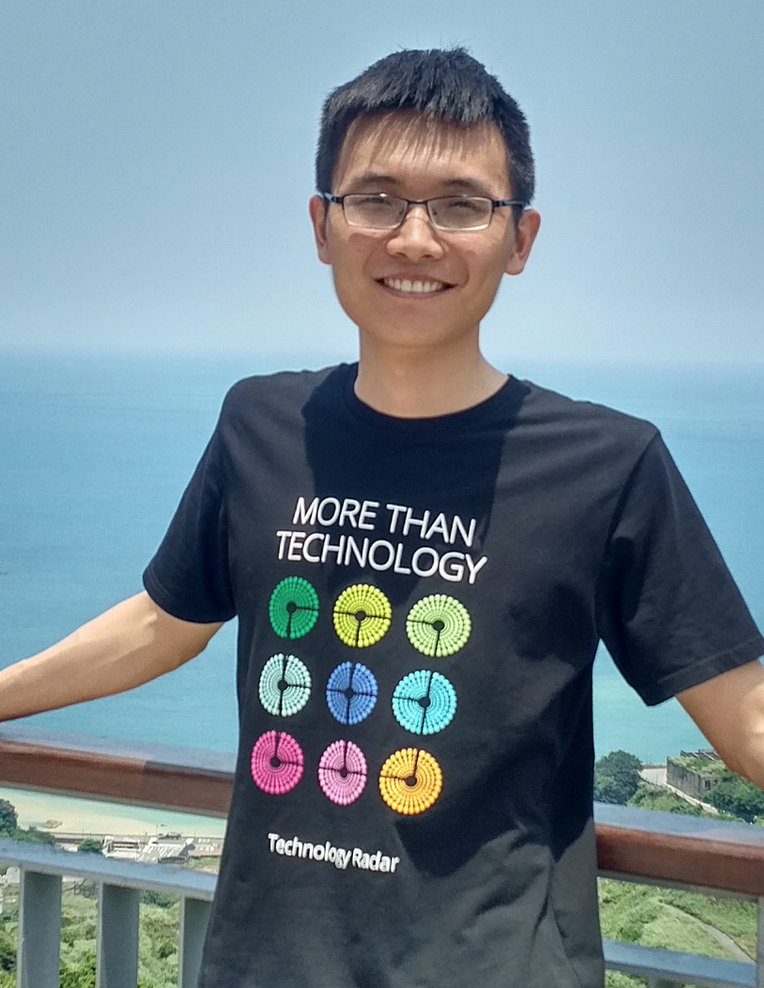
\includegraphics[width=0.7\columnwidth]{photo}
	\vspace{-7cm}
\end{figure}
\begin{flushright}\footnotesize
.\\
\vskip 6cm
\raggedright
\CVItem{{\large 个人信息:}}\\
电子邮件:\\
	\href{mailto:lc1990linux@gmail.com}{lc1990linux@gmail.com}  \\
	个人主页:\\
	\href{http://linchen2chris.github.io/}{linchen2chris.github.io} \\
	手机:\\ 13540394019	
  
	\CVItem{{\large 语言能力:}}\\
  \SmallSep
	\textit{\textbf{中文}:母语 \\\textbf{英语}:流利,常年与海外工程师一起工作\\}
	
  \vskip 1cm
  \CVItem{{\large 教育背景:}}\\
  \SmallSep
	\textit{2011-2014 四川大学-硕士: \textbf{计算机科学与技术}\\
    2007-2011 四川大学-本科: \textbf{公共管理+金融双学位}}

\end{flushright}\normalsize
\framebreak


% Right frame 右边内容在此定义
%%%%%%%%%%%%%%%%%%%%
\Huge\bfseries {\color{\myThemeColor} 林~~晨}\\
\normalsize\normalfont

% Skills
\CVSection{专业技能}
\hrule
\SmallSep
\CVItem{前端相关}\\
\textit{$\bullet$ 熟悉react, flutter} \\
\\
\CVItem{后端相关}\\
\textit{$\bullet$ 熟悉nodejs, golang} \\
\\
\CVItem{Devops}\\
\textit{$\bullet$ 熟悉AWS, GCP常用服务,Terraform,K8s}\\

\CVItem{其它}\\
\textit{$\bullet$ 熟悉CI/CD, Agile, Scrum,TDD等开发方法}\\
\\

% Experience
\CVSection{工作经历}
\hrule
\SmallSep
\CVItem{2016.10 - 至今: 担任软件工程师,Tech Lead \hfill ThoughtWorks}\\

\textit{$\bullet$ 2022.3-至今: 全球Top1口腔医疗软件PaaS平台} \\
\textit{$\bullet$ 职责: 1.使用golang 和flutter 参与无线口扫设备的软件开发 2.同时负责GCP/K8s上的应用部署 }\\

\textit{$\bullet$ 2021.9-2022.3: 新加坡国民应用运维} \\
\textit{$\bullet$ 职责: 根据新需求开发和维护线上应用, 并应用terraform把应用部署到AWS上}\\

\textit{$\bullet$ 2021.2-2021.9: 澳洲地产公司REA数据平台} \\
\textit{$\bullet$ 职责:
  1. 运维 REA 在AWS上的用户系统
  2. 带领团队使用airflow从AWS和Salesforce上迁移并清洗数据到GCP,在GCP上建立数据市场供公司内部使用,用清洗后的数据反哺应用。}\\

\textit{$\bullet$ 2020.9-2021.2:国内Top1商业银行低代码平台} \\
\textit{$\bullet$ 职责: 带领前端团队使用React构建低代码平台的前端部分, 实现低代码应用的设计页面和运行时} \\

\textit{$\bullet$ 2020.1-2020.9:澳洲会计公司MYOB的应用表单} \\
\textit{$\bullet$ 职责: 带领团队使用React+Nodejs, 大量使用AWS云服务如stepFunction, Lambda, cloudformation,SES 搭建一个应用表单系统, 非技术人员可以快速构建一个内部表单用于收集数据, 触发邮件通知, 审批流程} \\

\textit{$\bullet$ 2018.8-2020.1:新加坡国民应用开发} \\
\textit{$\bullet$ 职责: 在新加坡带领团队搭建CMS系统, 使用React, Nodejs, Elastic Search, AWS ECS等服务 } \\

\textit{$\bullet$ 2016.10-2018.8: 澳洲金融机构Suncorp的网上保险和银行应用开发} \\
\textit{$\bullet$ 职责: 使用react 构建前端应用, Sprint Boot构建微服务应用, 在这个项目上接触到了大量敏捷软件开发实践和Devops实践, 极大改变了我之后软件开发的职业生涯, 从此我开始实践TDD, 微服务架构, 持续交付, 持续部署, 蓝绿部署} \\

\CVItem{2015.10 - 2016.10 \hfill 创业}\\
\textit{$\bullet$ 医院血透管理系统} \\
\textit{$\bullet$ 项目技术栈:后端采用~nodejs + mongodb~, 前端采用~react+redux~, 病人移动端采用 Android和iOS} \\
\textit{$\bullet$ 项目通过患者移动端,和医院~web~端协同工作,实现肾病患者的全周期管理。}\\
\\
\CVItem{2014.07 - 2015.10 \hfill 瞬联科技}\\
\textit{$\bullet$ 担任后端工程师,维护电信后台计费系统} \\
\textit{$\bullet$ 项目主要采用C/C++, 基于Unix服务器开发,熟悉unix工具链和开发环境, 所在小组参与了实时计费系统和后计费系统的整合。} \\

\end{CJK*}
\end{document}
